\documentclass[10pt]{beamer}
\usetheme{metropolis}
\usepackage{booktabs}
\usepackage{tabularx}
\usepackage{calc}
\usepackage{tikz}
\usepackage{fontawesome5}
\usetikzlibrary{shapes.geometric,patterns}

% Setup for faculty images
\newlength{\imageheight}
\setlength{\imageheight}{3.5cm}

% Define CSUF brand colors
\definecolor{titanblue}{HTML}{00244E}
\definecolor{mediumblue}{HTML}{0F3F8C}
\definecolor{skyblue}{HTML}{EBFBFF}
\definecolor{titanorange}{HTML}{FF7900}
\definecolor{titangray}{HTML}{F5F5F5}
\definecolor{titantext}{HTML}{222222}

% Additional vibrant colors
\definecolor{successcolor}{HTML}{27AE60}
\definecolor{infocolor}{HTML}{3498DB}
\definecolor{warningcolor}{HTML}{F39C12}
\definecolor{accentcolor}{HTML}{9B59B6}
\definecolor{dangercolor}{HTML}{E74C3C}

% Customize metropolis theme colors
\setbeamercolor{normal text}{fg=titantext, bg=white}
\setbeamercolor{alerted text}{fg=titanorange}
\setbeamercolor{example text}{fg=mediumblue}

% Title page colors
\setbeamercolor{title}{fg=titanblue, bg=white}
\setbeamercolor{subtitle}{fg=mediumblue, bg=white}
\setbeamercolor{institute}{fg=titanorange, bg=white}
\setbeamercolor{date}{fg=titanblue, bg=white}

% Frame title colors
\setbeamercolor{frametitle}{fg=white, bg=titanblue}
\setbeamercolor{framesubtitle}{fg=mediumblue, bg=white}

% Block environment colors
\setbeamercolor{block title}{fg=white, bg=titanblue}
\setbeamercolor{block body}{fg=titantext, bg=skyblue!10}

% Different block types
\setbeamercolor{block title example}{fg=white, bg=successcolor}
\setbeamercolor{block body example}{fg=titantext, bg=successcolor!10}

\setbeamercolor{block title alerted}{fg=white, bg=infocolor}
\setbeamercolor{block body alerted}{fg=titantext, bg=infocolor!10}

% Item colors
\setbeamercolor{itemize item}{fg=titanorange}
\setbeamercolor{itemize subitem}{fg=mediumblue}
\setbeamercolor{itemize subsubitem}{fg=titanblue}

% Footer and header colors
\setbeamercolor{footer}{fg=titantext}
\setbeamercolor{header}{fg=titanblue}

% Customize fonts
\setbeamerfont{title}{size=\Large, series=\bfseries}
\setbeamerfont{frametitle}{size=\large, series=\bfseries}

% Custom section slide template
\defbeamertemplate{background}{section}{%
\begin{tikzpicture}[remember picture,overlay]
\fill[titanorange,opacity=0.8] (current page.south west) rectangle (current page.north east);
\end{tikzpicture}
}

% Simple title page template
\defbeamertemplate*{title page}{customized}[1][]
{
\vspace{1cm}
 {\usebeamerfont{title}\usebeamercolor[fg]{title}\inserttitle\par}
\vspace{0.5cm}
 {\usebeamerfont{subtitle}\usebeamercolor[fg]{subtitle}\insertsubtitle\par}
\vspace{0.5cm}
 {\usebeamerfont{date}\usebeamercolor[fg]{date}\insertdate\par}
\vfill
 {\insertinstitute\par}
}

% Add progress bar
\makeatletter
\setbeamertemplate{headline}{%
\begin{beamercolorbox}[wd=\paperwidth,ht=0.4cm,dp=0cm]{titanblue}%
\begin{tikzpicture}
\fill[titanorange] (0,0) rectangle (\the\paperwidth*\insertframenumber/\inserttotalframenumber,0.4cm);
\end{tikzpicture}%
\end{beamercolorbox}%
}
\makeatother

\begin{document}

\title{Federalism and Public Policy}
\subtitle{Power Distribution in American Governance\\POSC 315: Introduction to Public Policy\\Lecture 3.2}
\date{Summer 2025}
\institute{California State University, Fullerton}

\maketitle

% Section: What is Federalism?
{
\setbeamertemplate{background}[section]
\begin{frame}[plain]
\vspace{2cm}
\begin{center}
{\Huge\color{white}\textbf{What is Federalism?}}
\end{center}
\end{frame}
}

% Federalism Defined
\begin{frame}
\frametitle{Federalism Defined}

\begin{alertblock}{Definition}
\textbf{Federalism}: The division of power between a central government and regional governments

\vspace{0.3cm}
\emph{The distribution of power and authority on a geographical basis}.
\end{alertblock}

\end{frame}

% Core Features
\begin{frame}
\frametitle{Core Features}

\begin{itemize}
\item<1-> A system of checks and balances between the national and state governments
\item<2-> The founders believed that federalism would protect liberty
\item<3-> Protects against \textcolor{warningcolor}{\textbf{factions}}: groups of citizens who have a common interest in some proposal that would either violate the rights of other citizens or harm the nation
\end{itemize}

\end{frame}

% The Founders' View
\begin{frame}
\frametitle{The Founders' View}

\begin{columns}
\begin{column}{0.48\textwidth}
\begin{block}{Governance Benefits}
\pause
\begin{itemize}
\item Prevents faction dominance
\item State policy experimentation
\item Government closer to people
\end{itemize}
\end{block}
\end{column}

\begin{column}{0.48\textwidth}
\begin{block}{Democratic Benefits}
\pause
\begin{itemize}
\item Increases political participation
\item More effective government
\item More access points to government
\item Increases policy innovation
\end{itemize}
\end{block}
\end{column}
\end{columns}

\end{frame}

% Eras of Federalism (Book)
\begin{frame}
\frametitle{Eras of Federalism}
\framesubtitle{(from the Textbook)}

\begin{center}
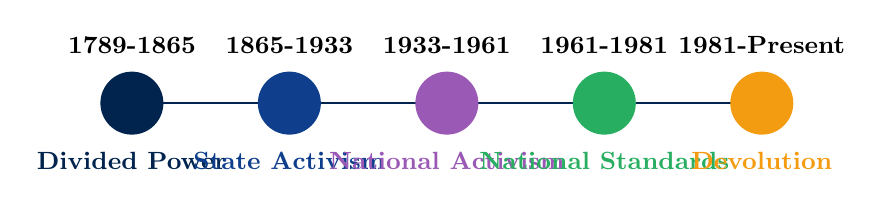
\begin{tikzpicture}[scale=0.8, every node/.style={align=center}]
% Timeline base
\draw[thick, titanblue] (0,0) -- (10,0);

% Era 1
\node[circle, fill=titanblue, text=white, minimum size=0.8cm] at (0,0) {};
\node[above=0.5cm] at (0,0) {\small\textbf{1789-1865}};
\node[below=0.5cm, text=titanblue] at (0,0) {\small\textbf{Divided Power}};

% Era 2
\node[circle, fill=mediumblue, text=white, minimum size=0.8cm] at (2.5,0) {};
\node[above=0.5cm] at (2.5,0) {\small\textbf{1865-1933}};
\node[below=0.5cm, text=mediumblue] at (2.5,0) {\small\textbf{State Activism}};

% Era 3
\node[circle, fill=accentcolor, text=white, minimum size=0.8cm] at (5,0) {};
\node[above=0.5cm] at (5,0) {\small\textbf{1933-1961}};
\node[below=0.5cm, text=accentcolor] at (5,0) {\small\textbf{National Activism}};

% Era 4
\node[circle, fill=successcolor, text=white, minimum size=0.8cm] at (7.5,0) {};
\node[above=0.5cm] at (7.5,0) {\small\textbf{1961-1981}};
\node[below=0.5cm, text=successcolor] at (7.5,0) {\small\textbf{National Standards}};

% Era 5
\node[circle, fill=warningcolor, text=white, minimum size=0.8cm] at (10,0) {};
\node[above=0.5cm] at (10,0) {\small\textbf{1981-Present}};
\node[below=0.5cm, text=warningcolor] at (10,0) {\small\textbf{Devolution}};
\end{tikzpicture}
\end{center}

\end{frame}

% Section: Models of Federalism
{
\setbeamertemplate{background}[section]
\begin{frame}[plain]
\vspace{2cm}
\begin{center}
{\Huge\color{white}\textbf{Models of Federalism}}

\vspace{0.5cm}
{\large\color{white}(from the Literature)}
\end{center}
\end{frame}
}

% Five Models Progress Bar
\begin{frame}
\frametitle{Five Models of Federalism}

\begin{center}
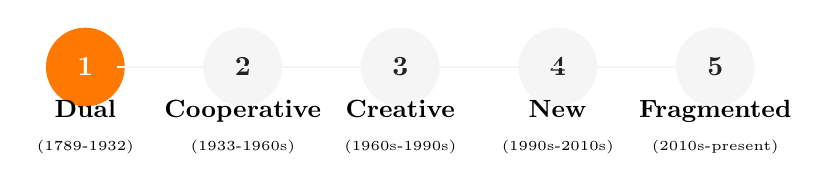
\begin{tikzpicture}[scale=0.8]
% Draw progress steps
\foreach \x/\num/\label/\years/\active in {0/1/Dual/1789-1932/1, 2.5/2/Cooperative/1933-1960s/0, 5/3/Creative/1960s-1990s/0, 7.5/4/New/1990s-2010s/0, 10/5/Fragmented/2010s-present/0} {
    \ifnum\active=1
        \node[circle, fill=titanorange, text=white, minimum size=1cm] at (\x,1) {\textbf{\num}};
    \else
        \node[circle, fill=titangray, text=titantext, minimum size=1cm] at (\x,1) {\textbf{\num}};
    \fi
    \node[below=0.3cm, align=center] at (\x,1) {\small\textbf{\label}};
    \node[below=0.8cm, align=center] at (\x,1) {\tiny(\years)};
}

% Connect the circles
\draw[thick, titangray] (0.5,1) -- (9.5,1);
\end{tikzpicture}
\end{center}

\end{frame}

% Dual Federalism with Visual
\begin{frame}
\frametitle{Dual Federalism \textcolor{mediumblue}{(1789-1932)}}

\begin{columns}
\begin{column}{0.4\textwidth}
\begin{center}
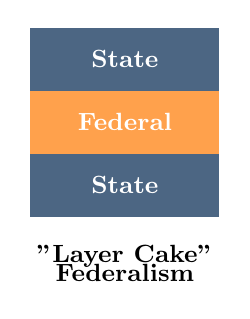
\begin{tikzpicture}[scale=0.8]
% Draw layer cake
\fill[titanblue!70] (0,0) rectangle (3,1);
\fill[titanorange!70] (0,1) rectangle (3,2);
\fill[titanblue!70] (0,2) rectangle (3,3);

% Labels
\node[white] at (1.5,0.5) {\small\textbf{State}};
\node[white] at (1.5,1.5) {\small\textbf{Federal}};
\node[white] at (1.5,2.5) {\small\textbf{State}};

% Title
\node[below] at (1.5,-0.3) {\small\textbf{"Layer Cake"}};
\node[below] at (1.5,-0.6) {\small\textbf{Federalism}};
\end{tikzpicture}
\end{center}
\end{column}

\begin{column}{0.6\textwidth}
\begin{itemize}
\item<1-> \textbf{Clear division of authority}
\item<2-> \textbf{National government is supreme in its sphere}
\item<3-> \textbf{Little overlap between the two spheres}
\item<4-> \textbf{National government is limited to enumerated powers}
\item<5-> \textbf{Overall: State-centered federalism}
\end{itemize}
\end{column}
\end{columns}

\end{frame}

% Cooperative Federalism with Visual
\begin{frame}
\frametitle{Cooperative Federalism \textcolor{mediumblue}{(1933-1960s)}}

\begin{columns}
\begin{column}{0.4\textwidth}
\begin{center}

\begin{tikzpicture}[scale=0.8]
% Draw marble cake pattern
\fill[titanblue!70] (0,0) rectangle (3,3);
\fill[titanorange!70] (0.2,0.2) rectangle (2.8,0.8);
\fill[titanorange!70] (0.3,1.3) rectangle (2.7,1.9);
\fill[titanorange!70] (0.1,2.1) rectangle (2.9,2.7);

% Irregular patterns to simulate marble
\fill[titanorange!70] (0.5,0.9) rectangle (1.5,1.2);
\fill[titanorange!70] (1.8,0.3) rectangle (2.4,0.6);

% Title
\node[below] at (1.5,-0.3) {\small\textbf{"Marble Cake"}};
\node[below] at (1.5,-0.6) {\small\textbf{Federalism}};
\end{tikzpicture}
\end{center}
\end{column}

\begin{column}{0.6\textwidth}
\begin{itemize}
\item<1-> \textbf{National and state governments share powers}
\item<2-> \textbf{Federal powers expand to deal with the Great Depression}
\item<3-> \textbf{Cooperation between national and state governments}
\item<4-> \textbf{Overall: National-centered federalism}
\end{itemize}
\end{column}
\end{columns}

\end{frame}

% Creative Federalism with Visual
\begin{frame}
\frametitle{Creative Federalism \textcolor{mediumblue}{(1960s-1990s)}}

\begin{columns}
\begin{column}{0.4\textwidth}
\begin{center}

\begin{tikzpicture}[scale=0.8]
% Draw picket fence
\foreach \x in {0.3,0.9,1.5,2.1,2.7} {
    \fill[titanblue] (\x,0) rectangle (\x+0.2,3);
}
% Horizontal rails
\fill[titanorange] (0,1) rectangle (3,1.3);
\fill[titanorange] (0,2) rectangle (3,2.3);

% Title
\node[below] at (1.5,-0.3) {\small\textbf{"Picket Fence"}};
\node[below] at (1.5,-0.6) {\small\textbf{Federalism}};
\end{tikzpicture}
\end{center}
\end{column}

\begin{column}{0.6\textwidth}
\begin{itemize}
\item<1-> \textbf{Great Society programs}
\item<2-> \textbf{National government sets policy goals}
\item<3-> \textbf{States implement policy}
\item<4-> \textbf{Creative use of grants-in-aid}
\item<5-> \textbf{Overall: National-centered federalism}
\end{itemize}
\end{column}
\end{columns}

\end{frame}

% New Federalism with Visual
\begin{frame}
\frametitle{New Federalism \textcolor{mediumblue}{(1990s-2010s)}}

\begin{columns}
\begin{column}{0.4\textwidth}
\begin{center}
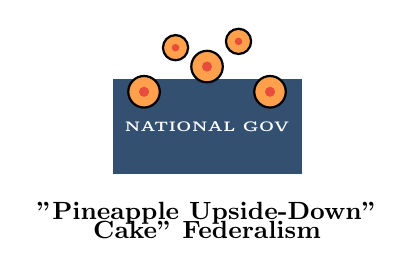
\begin{tikzpicture}[scale=0.8]
% Draw the cake base (National Government)
\fill[titanblue!80] (0,0) rectangle (3,1.5);
\node[white, font=\tiny] at (1.5,0.75) {\textbf{NATIONAL GOV}};

% Draw pineapple rings (State Governments) on top
\draw[thick, fill=titanorange!70] (0.5,1.3) circle (0.25);
\draw[thick, fill=titanorange!70] (1.5,1.7) circle (0.25);
\draw[thick, fill=titanorange!70] (2.5,1.3) circle (0.25);

% Draw cherries (Local Governments) inside pineapples
\fill[dangercolor] (0.5,1.3) circle (0.08);
\fill[dangercolor] (1.5,1.7) circle (0.08);
\fill[dangercolor] (2.5,1.3) circle (0.08);

% Add some extra pineapples
\draw[thick, fill=titanorange!70] (1,2) circle (0.2);
\fill[dangercolor] (1,2) circle (0.06);
\draw[thick, fill=titanorange!70] (2,2.1) circle (0.2);
\fill[dangercolor] (2,2.1) circle (0.06);

% Title
\node[below] at (1.5,-0.3) {\small\textbf{"Pineapple Upside-Down"}};
\node[below] at (1.5,-0.6) {\small\textbf{Cake" Federalism}};
\end{tikzpicture}
\end{center}
\end{column}

\begin{column}{0.6\textwidth}
\begin{itemize}
\item<1-> \textbf{Competitive Federalism}
\item<2-> \textbf{Devolution Revolution}
\item<3-> \textbf{National government returns power to the states}
\item<4-> \textbf{Block grants}
\item<5-> \textbf{Overall: State-centered federalism}
\end{itemize}
\end{column}
\end{columns}

\end{frame}

% Fragmented Federalism
\begin{frame}
\frametitle{Fragmented Federalism \textcolor{mediumblue}{(2010s-present)}}

\begin{center}
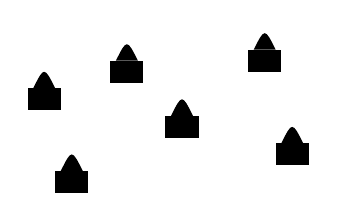
\begin{tikzpicture}[scale=0.7]
% Draw scattered cupcakes
\foreach \x/\y/\color in {1/1/titanblue, 3/2/titanorange, 5/1.5/successcolor, 2/3/warningcolor, 4.5/3.2/accentcolor, 0.5/2.5/mediumblue} {
    % Cupcake base
    \fill[\color!70] (\x-0.3,\y-0.3) rectangle (\x+0.3,\y+0.1);
    % Frosting
    \fill[\color] (\x-0.2,\y+0.1) .. controls (\x,\y+0.5) .. (\x+0.2,\y+0.1);
}
\end{tikzpicture}
\end{center}

\begin{itemize}
\item<1-> \textbf{"Cupcake Federalism"}
\item<2-> \textbf{Federalism is a mess}
\item<3-> \textbf{Federal government is pursuing state-specific policies}
\item<4-> \textbf{States are pursuing policies with little federal direction}
\item<5-> \textbf{Federalism is fractured: dimensions of all previous models}
\item<6-> \textbf{Overall: ???-centered federalism}
\end{itemize}

\end{frame}

% Section: Federalism in Practice
{
\setbeamertemplate{background}[section]
\begin{frame}[plain]
\vspace{1.5cm}
\begin{center}
{\Huge\color{white}\textbf{Federalism in Practice}}

\vspace{0.5cm}
{\large\color{white}Policy Implementation in a Federal System}
\end{center}
\end{frame}
}

% Policy Laboratories
\begin{frame}
\frametitle{Policy Laboratories}

\pause
\begin{quotation}
``It is one of the happy incidents of the federal system that a single courageous State may, if its citizens choose, serve as a laboratory; and try novel social and economic experiments without risk to the rest of the country.''

\vspace{0.5cm}
\hfill --- Justice Louis Brandeis (1932)
\end{quotation}

\end{frame}

% State Policy Innovation
\begin{frame}
\frametitle{State Policy Innovation}

\begin{columns}
\begin{column}{0.32\textwidth}
\begin{center}

\begin{tikzpicture}[scale=0.8]
\node[circle, fill=infocolor, text=white, minimum size=1.5cm] at (0,0) {\Large\faMicroscope};
\end{tikzpicture}

\textbf{State Laboratories}

States experiment with different policy approaches
\end{center}
\end{column}

\begin{column}{0.32\textwidth}
\begin{center}

\begin{tikzpicture}[scale=0.8]
\node[circle, fill=successcolor, text=white, minimum size=1.5cm] at (0,0) {\Large\faSync};
\end{tikzpicture}

\textbf{Policy Diffusion}

Successful policies spread across states
\end{center}
\end{column}

\begin{column}{0.32\textwidth}
\begin{center}

\begin{tikzpicture}[scale=0.8]
\node[circle, fill=warningcolor, text=white, minimum size=1.5cm] at (0,0) {\Large\faChartBar};
\end{tikzpicture}

\textbf{Comparative Analysis}

Which approaches work best?
\end{center}
\end{column}
\end{columns}

\end{frame}

% Federal-State Coordination
\begin{frame}
\frametitle{Federal-State Coordination}

\begin{columns}
\begin{column}{0.48\textwidth}
\begin{block}{Federal Tools}
\pause
\begin{itemize}
\item Categorical grants
\item Block grants
\item Mandates
\item Regulatory frameworks
\end{itemize}
\end{block}
\end{column}

\begin{column}{0.48\textwidth}
\begin{block}{State Implementation}
\pause
\begin{itemize}
\item Administrative adaptation
\item Supplemental funding
\item Waiver requests
\item Local distribution
\end{itemize}
\end{block}
\end{column}
\end{columns}

\end{frame}

% Conclusion
{
\setbeamertemplate{background}[section]
\begin{frame}[plain]
\vspace{1.5cm}
\begin{center}
{\Huge\color{white}\textbf{Understanding Federalism}}

\vspace{0.8cm}
{\Large\color{white}Is Key to Understanding American Policy}
{\Large\color{white}Design and Implementation}
\end{center}
\end{frame}
}

\end{document}